\documentclass[a4paper,12pt]{article}

\usepackage{cite}
\usepackage{amsmath,amssymb,amsfonts}
\usepackage{algorithmic}
\usepackage{graphicx}
\usepackage{textcomp}
\usepackage{xcolor}
\usepackage{booktabs}
\usepackage{url}
\def\BibTeX{{\rm B\kern-.05em{\sc i\kern-.025em b}\kern-.08em
    T\kern-.1667em\lower.7ex\hbox{E}\kern-.125emX}}
\begin{document}

\title{Assignment 3: Planning and Scheduling, and Neural Networks %\\
%{\footnotesize \textsuperscript{*}Note: Sub-titles are not captured for https://ieeexplore.ieee.org  and
%should not be used}
%\thanks{Identify applicable funding agency here. If none, delete this.}
}

\author{Renjiro Owen\\
\textit{Victoria University Wellington}\\
Wellington, New Zealand\\
owenrenj@myvuw.ac.nz}

\maketitle
\section{Job Shop Scheduling}

The Job Shop Scheduling problem considered in this work consists of three jobs, $J_1$, $J_2$, and $J_3$, processed on two machines, $M_1$ and $M_2$. Each job has two operations that must be completed in a specified order, with different arrival and processing times, as shown in Table~\ref{tab:jss}. An operation can only start after its job has arrived and, for the second operation of a job, after the previous operation has been completed. In addition, each machine can process only one operation at a time. The objective is to determine the starting time of each operation while satisfying these constraints.

\begin{table}[ht]
	\centering
	\caption{Job Shop Scheduling Problem}
	\label{tab:jss}
	\begin{tabular}{c c c c c}
		\hline
		\textbf{Job} & \textbf{Arrival Time} & \textbf{Operation} & \textbf{Machine} & \textbf{Proc. Time} \\
		\hline
		$J_1$ & 0  & $O_{11}$ & $M_1$ & 50 \\
		&    & $O_{12}$ & $M_2$ & 25 \\
		$J_2$ & 10 & $O_{21}$ & $M_2$ & 30 \\
		&    & $O_{22}$ & $M_1$ & 35 \\
		$J_3$ & 20 & $O_{31}$ & $M_1$ & 40 \\
		&    & $O_{32}$ & $M_2$ & 20 \\
		\hline
	\end{tabular}
\end{table}

\subsection{Earliest Starting Times}

Given the specified action sequence, the earliest starting time of each operation is determined by taking the later of the operation's ready time and the machine's available time. The resulting starting times are shown in Table~\ref{tab:earliest-start}.

\begin{table}[ht]
	\centering
	\caption{Earliest starting times for the given action sequence}
	\label{tab:earliest-start}
	\begin{tabular}{c c c c c}
		\hline
		\textbf{Action} & \textbf{Ready Time} & \textbf{Machine Available} & \textbf{Start} & \textbf{Finish} \\
		\hline
		$O_{11}$ on $M_1$ & 0  & 0  & $t_1=0$  & 50 \\
		$O_{21}$ on $M_2$ & 10 & 0  & $t_2=10$ & 40 \\
		$O_{31}$ on $M_1$ & 20 & 50 & $t_3=50$ & 90 \\
		$O_{12}$ on $M_2$ & 50 & 40 & $t_4=50$ & 75 \\
		$O_{22}$ on $M_1$ & 40 & 90 & $t_5=90$ & 125 \\
		$O_{32}$ on $M_2$ & 90 & 75 & $t_6=90$ & 110 \\
		\hline
	\end{tabular}
\end{table}

Therefore, the earliest starting times are

$$
(t_1,t_2,t_3,t_4,t_5,t_6)=(0,10,50,50,90,90).
$$

\subsection{Job Completion Time and Makespan}

Using the schedule from Question 1, the completion time of each job is the finishing time of its last operation. Thus, $J_1$ finishes after $O_{12}$ at time 75, $J_2$ finishes after $O_{22}$ at time 125, and $J_3$ finishes after $O_{32}$ at time 110. The completion times and makespan are shown below.

\begin{table}[ht]
	\centering
	\caption{Job completion times}
	\label{tab:completion-times}
	\begin{tabular}{c c c}
		\hline
		\textbf{Job} & \textbf{Last Operation} & \textbf{Completion Time} \\
		\hline
		$J_1$ & $O_{12}$ & 75 \\
		$J_2$ & $O_{22}$ & 125 \\
		$J_3$ & $O_{32}$ & 110 \\
		\hline
	\end{tabular}
\end{table}

Therefore, the makespan is the maximum completion time:

$$
C_{\max} = \max(75,125,110) = 125.
$$
\subsection{SPT Dispatching Rule}

The Shortest Processing Time (SPT) dispatching rule selects the available operation with the shortest processing time whenever a machine becomes available. Applying SPT to the given jobs produces the following schedule:

\begin{table}[ht]
	\centering
	\caption{SPT schedule}
	\label{tab:spt-schedule}
	\begin{tabular}{c c c c c}
		\hline
		\textbf{Job} & \textbf{Operation} & \textbf{Machine} & \textbf{Start} & \textbf{Finish} \\
		\hline
		$J_1$ & $O_{11}$ & $M_1$ & 0   & 50 \\
		$J_2$ & $O_{21}$ & $M_2$ & 10  & 40 \\
		$J_2$ & $O_{22}$ & $M_1$ & 50  & 85 \\
		$J_1$ & $O_{12}$ & $M_2$ & 50  & 75 \\
		$J_3$ & $O_{31}$ & $M_1$ & 85  & 125 \\
		$J_3$ & $O_{32}$ & $M_2$ & 125 & 145 \\
		\hline
	\end{tabular}
\end{table}

Therefore, the final SPT solution has a makespan of

$$
C_{\max}=145.
$$

\subsection{SPT Completion Times and Makespan}

Using the SPT schedule from the previous question, the completion time of each job is the finishing time of its last operation. Therefore, $J_1$ completes at time 75, $J_2$ at time 85, and $J_3$ at time 145. The makespan is the maximum completion time:

$$
C_{\max}^{\mathrm{SPT}} = \max(75,85,145)=145.
$$

For the FCFS solution from Question 1, the completion times are $J_1=115$, $J_2=125$, and $J_3=135$, giving a makespan of

$$
C_{\max}^{\mathrm{FCFS}} = \max(115,125,135)=135.
$$

Thus, the two solutions have makespans of 145 for SPT and 135 for FCFS, respectively. The difference in makespan is

$$
145-135=10.
$$

Hence, based solely on makespan, the FCFS schedule has a 10-time-unit smaller makespan than the SPT schedule.

\subsection{Comparison of SPT and FCFS}

The two solutions are generated using the SPT and FCFS dispatching rules, respectively. Although the FCFS solution has a smaller overall makespan of 135 compared with 145 for SPT, SPT provides earlier completion times for $J_1$ and $J_2$. Under SPT, $J_1$ and $J_2$ finish at times 75 and 85, compared with 115 and 125 under FCFS. However, $J_3$ finishes later under SPT, at time 145 compared with 135 under FCFS.

Therefore, the performance of the two rules differs depending on the job being considered. This also shows that a smaller completion time for some jobs does not necessarily result in a smaller overall makespan. The performance of a dispatching rule depends on the specific job data, processing times, arrival times, and machine constraints.

\subsection{Methods for Job Shop Scheduling}

Two methods can be used to handle the job shop scheduling problem under static and dynamic conditions. For the static case, where all jobs and processing times are known in advance, a Genetic Algorithm (GA) can be used to minimise the makespan. Each chromosome represents an operation sequence, with each job appearing once for each of its operations. The sequence is decoded into a feasible schedule while satisfying operation precedence and machine capacity constraints. Tournament selection can select promising solutions, while crossover exchanges parts of two parent sequences and mutation can swap or move operations. The fitness of each solution is evaluated using its makespan, and the process is repeated for a fixed number of generations.

For the dynamic case, a rolling-horizon re-optimisation approach can be used. At each decision point, the current machine status and all currently known jobs are used to generate a new schedule. Operations that have already started remain fixed, while unscheduled operations can be changed. When a new job arrives or a machine becomes available, the scheduling process is repeated using the updated information. The same operation-based representation and search operators can be used, allowing the schedule to adapt to unexpected job arrivals and changing machine availability.


\section{Neural Networks}
\subsection{Training a Simple Perceptron on Linearly Separable Data}

A simple perceptron was implemented from scratch using NumPy to perform binary classification on the SeaSyn dataset. The training set, \texttt{SeaSynTrain.csv}, was used to train the model, while \texttt{SeaSynTest.csv} was used to evaluate its performance. The three continuous attributes, \texttt{attrib1}, \texttt{attrib2}, and \texttt{attrib3}, were used as input features, with the \texttt{class} column representing the binary target variable. The perceptron used a learning rate of 0.01 and a step activation function. Initially, the weights and bias were set to zero. For each training sample, the prediction error was calculated and used to update the weights and bias according to the perceptron learning rule.

The perceptron was trained using different numbers of epochs to investigate how training duration affects classification accuracy. Accuracy was calculated as the proportion of correctly classified samples. The resulting training and test accuracies are shown in Table~\ref{tab:perceptron_results}.

\begin{table}[ht]
	\centering
	\caption{Perceptron accuracy for different numbers of training epochs.}
	\label{tab:perceptron_results}
	\begin{tabular}{c|c|c}
		\hline
		\textbf{Epochs} & \textbf{Training Accuracy} & \textbf{Test Accuracy} \\
		\hline
		1   & 0.6500 & 0.6250 \\
		5   & 0.7500 & 0.7000 \\
		10  & 0.6900 & 0.6000 \\
		15  & 0.8500 & 0.8500 \\
		20  & 0.7200 & 0.6250 \\
		50  & 0.7300 & 0.6500 \\
		60  & 0.7100 & 0.6000 \\
		80  & 0.7000 & 0.6250 \\
		100 & 0.7200 & 0.6250 \\
		120 & 0.7500 & 0.6750 \\
		150 & 0.7900 & 0.7500 \\
		200 & 0.8100 & 0.7500 \\
		\hline
	\end{tabular}
\end{table}

The results show that increasing the number of epochs does not produce a consistent increase in test accuracy. For example, the test accuracy increases from 0.625 at one epoch to 0.700 at five epochs and reaches its highest observed value of 0.850 at 15 epochs. However, it then decreases to 0.600 at 60 epochs before gradually increasing again to 0.750 at 150 and 200 epochs. Therefore, training for more epochs does not necessarily result in better generalisation on the test set.

The variation in accuracy is characteristic of the perceptron learning algorithm. The weights are updated whenever a training sample is misclassified, meaning that continued training can change the decision boundary rather than simply improving it monotonically. In these experiments, 15 epochs produced the highest test accuracy, with both training and test accuracy reaching 0.850. At 200 epochs, the training accuracy increased to 0.810, but the test accuracy was lower at 0.750. This indicates that a larger number of epochs did not improve the model's generalisation performance for this particular train-test split.

Overall, the results suggest that the number of epochs should not simply be increased indefinitely. A relatively small number of epochs was sufficient to obtain strong test performance, while additional training produced fluctuations in accuracy. For this experiment, 15 epochs gave the highest test-set accuracy among the tested values.

\subsection{Training a Simple Perceptron on Non-Linearly Separable Data}

The same perceptron implementation from Task (a) was reused to classify the RingSyn dataset. In this experiment, \texttt{RingSynTrain.csv} was used for training and \texttt{RingSynTest.csv} was used for evaluation. The dataset contains two continuous input features, \texttt{feature1} and \texttt{feature2}, and a binary target variable, \texttt{class}. The learning rate was set to 0.01, and the perceptron was trained using the same set of epoch values as in Task (a). Accuracy was used to measure the performance of the classifier.

The results are shown in Table~\ref{tab:ring_perceptron_results}.

\begin{table}[ht]
	\centering
	\caption{Perceptron accuracy on the RingSyn dataset for different numbers of epochs.}
	\label{tab:ring_perceptron_results}
	\begin{tabular}{c|c|c}
		\hline
		\textbf{Epochs} & \textbf{Training Accuracy} & \textbf{Test Accuracy} \\
		\hline
		1   & 0.6689 & 0.6567 \\
		5   & 0.6689 & 0.6567 \\
		10  & 0.7241 & 0.7200 \\
		15  & 0.6689 & 0.6567 \\
		20  & 0.6689 & 0.6567 \\
		50  & 0.7506 & 0.7500 \\
		60  & 0.6689 & 0.6567 \\
		80  & 0.6689 & 0.6567 \\
		100 & 0.6689 & 0.6567 \\
		120 & 0.6689 & 0.6567 \\
		150 & 0.6689 & 0.6567 \\
		200 & 0.6689 & 0.6567 \\
		\hline
	\end{tabular}
\end{table}

The perceptron performs relatively poorly on the RingSyn dataset compared with the linearly separable dataset used in Task (a). The highest test accuracy obtained was 0.7500 at 50 epochs, while most of the other epoch settings produced a test accuracy of approximately 0.6567. This indicates that increasing the number of epochs does not consistently improve the performance of the model.

The main reason for this behaviour is that the perceptron is a linear classifier. Its decision boundary has the form of a straight line, so it cannot effectively represent a circular or ring-shaped class boundary. Consequently, even with additional training epochs, the perceptron cannot find a decision boundary that correctly separates the classes. The changes in accuracy between different epoch settings are caused by the repeated weight updates as the algorithm encounters misclassified samples, rather than by the model learning a suitable non-linear boundary.

The results therefore demonstrate an important limitation of the perceptron. While it can perform well when the classes can be separated using a linear decision boundary, its performance is restricted when the underlying data distribution is non-linear. In this experiment, training for 50 epochs produced the highest observed test accuracy of 0.7500, but further increasing the number of epochs did not provide additional improvement. A model capable of learning non-linear decision boundaries would be more appropriate for this type of dataset.

\subsection{Training a MLP on Non-Linearly Separable Data}

To investigate whether a Multi-Layer Perceptron (MLP) can better handle the non-linearly separable RingSyn dataset, an MLP classifier from scikit-learn was used. The same training and test sets from Task (b) were used, with \texttt{feature1} and \texttt{feature2} as the input features and \texttt{class} as the target variable. The MLP used one hidden layer with ReLU activation and the Adam optimiser. The number of neurons in the hidden layer was tested from 4 to 10. A maximum of 10,000 training iterations was allowed to ensure that the model had sufficient opportunity to converge.

\begin{table}[ht]
	\centering
	\caption{MLP accuracy on the RingSyn dataset using different numbers of hidden neurons.}
	\label{tab:mlp_results}
	\begin{tabular}{c|c|c}
		\hline
		\textbf{Hidden Neurons} & \textbf{Training Accuracy} & \textbf{Test Accuracy} \\
		\hline
		4  & 0.9183 & 0.9133 \\
		5  & 0.9117 & 0.9333 \\
		6  & 0.9183 & 0.9233 \\
		7  & 0.9205 & 0.9233 \\
		8  & 0.9227 & 0.9233 \\
		9  & 0.9205 & 0.9433 \\
		10 & 0.9183 & 0.9100 \\
		\hline
	\end{tabular}
\end{table}

Figure~\ref{fig:mlp_performance} shows the training and test accuracy as the number of hidden neurons is increased. The test accuracy varies between 0.9100 and 0.9433. The highest test accuracy of 0.9433 was obtained using 9 hidden neurons. Increasing the number of neurons beyond this point did not improve performance, with the test accuracy decreasing to 0.9100 for 10 neurons. This demonstrates that increasing the size of the hidden layer does not necessarily result in better generalisation.

\begin{figure}[ht]
	\centering
	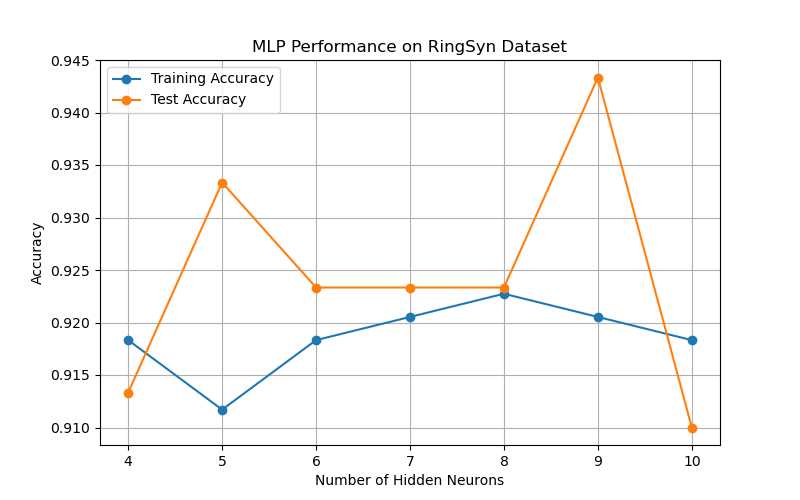
\includegraphics[width=0.8\linewidth]{../../MLPPerform.png}
	\caption{Training and test accuracy of the MLP for different numbers of hidden neurons.}
	\label{fig:mlp_performance}
\end{figure}

The MLP performed substantially better than the simple perceptron from Task (b). The perceptron achieved a highest test accuracy of 0.7500, obtained at 50 epochs, whereas the MLP achieved a test accuracy of 0.9433 using 9 hidden neurons. The MLP therefore correctly classified a considerably larger proportion of the test samples. Unlike the single-layer perceptron, the MLP contains a hidden layer that allows it to construct a non-linear decision boundary.

The improved performance indicates that the MLP was able to better capture the structure of the RingSyn dataset. A single perceptron can only produce a linear decision boundary, which limits its ability to separate classes arranged in a ring-like structure. The hidden layer of the MLP applies non-linear transformations to the input features, allowing the network to combine multiple decision boundaries into a more complex boundary. As a result, it can represent patterns that cannot be captured by a single linear classifier.

Overall, the experiment demonstrates the advantage of adding a hidden layer when dealing with non-linearly separable data. The MLP achieved substantially higher test accuracy than the perceptron, showing that the additional non-linear representation allowed it to capture more of the structure in the RingSyn dataset. Among the configurations tested, the MLP with 9 hidden neurons achieved the highest test accuracy of 0.9433.

\section*{Statement}

I declare that this assignment is my own work. The implementation, experimentation, model training, and evaluation were completed by me. Artificial intelligence Chatgpt\cite{chatgpt2026} were used only for language assistance during the preparation of this report.

\bibliographystyle{IEEEtran}   % or plain, unsrt, apalike, etc.
\bibliography{references}

\end{document}
